% 2. Nominal Interest Rates
% Stu Alden
%%%%%%%%%%%%%%%%%%%%%%%%%%%%%%%%%%%%%%%
\documentclass[14pt,twoside]{extarticle}
\usepackage{aldenarticle}
%%%%%%%%%%%%%%%%%%%%%%%%%%%%%%%%%%%%%%%
\begin{document}

\ArticleTitle{2. Nominal Interest Rates}

So far, we've  talked about interest rates that are compounded once per period, where the period is a year.

Since a year is a long time to wait, interest is often compounded more frequently than annually.  For example,
a bank might quote an interest rate of ``6\% per year, compounded monthly.''  This means that the interest is
actually being compounded 12 times per year, at a rate of 0.5\% (6\%/12) per \emph{month}.

The 6\% here is often called the \textbf{nominal} annual interest rate, because it is 6\% ``in name only.'' The
0.5\% is called the \textbf{effective} monthly interest rate, because it's the \emph{actual} rate that is being
applied to the balance each month. The nomenclature isn't great, but it's used all the time, so we need to get
comfortable with it.

The \textbf{effective annual rate} (sometimes called \textbf{EAR}) is the rate that would generate the same amount of interest if it were
compounded once per year.  In our 6\% monthly example, the EAR would be the rate $j$ that satisfies the equation
\[
  (1 + j) = (1 + 0.005)^{12}
\]

Solving for j we get 0.061678, or about 6.2\%.  Note that this effective annual rate is \emph{higher} than the
nominal rate (6\%), due to monthly (versus annual) compounding.

A year-long timeline might look like this:

\begin{center}
  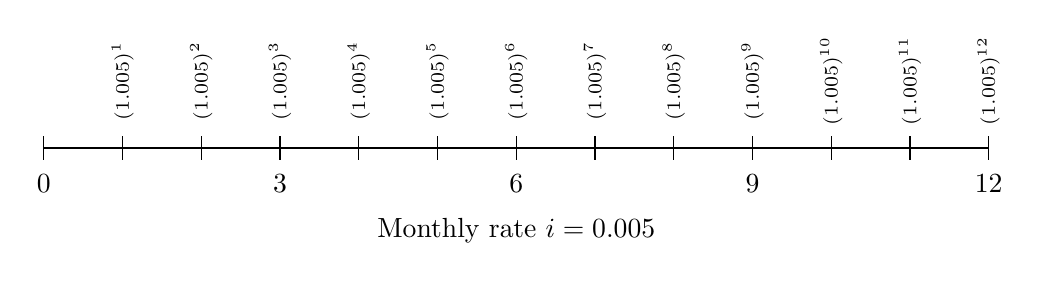
\begin{tikzpicture}[scale=1]

    % Main horizontal axis
    \draw[thick] (0,0) -- (12,0);

    % Tick marks
    \foreach \x in {0,...,12}
    \draw (\x,0.15) -- (\x,-0.15);

    % Month labels below axis
    \node[below=6pt] at (0,0) {0};
    \node[below=6pt] at (3,0) {3};
    \node[below=6pt] at (6,0) {6};
    \node[below=6pt] at (9,0) {9};
    \node[below=6pt] at (12,0) {12};

    % Monthly rate label
    \node[below=22pt] at (6,0)
    {Monthly rate $i = 0.005$};

    % Vertical accumulation factors
    \foreach \x in {1,...,12}
    \node[
      rotate=90,
      anchor=base,
      font=\scriptsize
    ] at (\x+0.08,0.85)
    {$ (1.005)^{\x} $};

  \end{tikzpicture}
\end{center}

\pagebreak

Monthly is perhaps the most common compounding frequency (conversion period), but you will see many
others, including semiannually (twice a year), quarterly (four times a year), and
\emph{daily}.

Although theoretical, it is very useful to think about \emph{continuous} compounding, where the conversion
period shrinks down to nothing!  At that point, we have the pure exponential growth you may recall from ``PERT''
problems in Algebra 2.  In calculus, you'll see the amazing connection, where

\[
  \lim_{n \to \infty} (1+\frac{j}{n})^n = e^j
\]

\textbf{Notes:}
\begin{itemize}
  \item For any choice of i) interest rate and ii) compounding period, an equivalent rate can be determined
        with a different rate and a different compounding period. So you can convert from annual to
        quarterly to daily to whatever you want.
  \item When doing financial math exercises, always start by identifying the \emph{period} and
        the corresponding effective \emph{rate per period}.
  \item For a given nominal rate, the more frequent the compounding, the higher the effective annual rate.

\end{itemize}

\end{document}
